\documentclass[11pt]{beamer}
\usepackage{listings} % Include the listings-package
\usepackage[T1]{fontenc}
\usepackage[utf8]{inputenc}
\usepackage[english]{babel}
\usepackage{amsmath}
\usepackage{amssymb, amsfonts, latexsym, cancel}
\usepackage{float}
\usepackage{graphicx}
\usepackage{epstopdf}
\usepackage{subfigure}
\usepackage{hyperref}
%\usepackage{authblk}
\usepackage{blindtext}
\usepackage{booktabs} % Allows the use of \toprule, 
\usepackage{filecontents}
\usepackage{courier} %% Sets font for listing as Courier.
\usepackage{listings}
%\usepackage{listings, xcolor}
\lstset{
tabsize = 2, %% set tab space width
showstringspaces = false, %% prevent space marking in strings, string is defined as the text that is generally printed directly to the console
numbers = left, %% display line numbers on the left
commentstyle = \color{green}, %% set comment color
keywordstyle = \color{blue}, %% set keyword color
stringstyle = \color{red}, %% set string color
rulecolor = \color{black}, %% set frame color to avoid being affected by text color
basicstyle = \small \ttfamily , %% set listing font and size
breaklines = true, %% enable line breaking
numberstyle = \tiny,
}
\usepackage{caption}
\DeclareCaptionFont{white}{\color{white}}
\DeclareCaptionFormat{listing}{\colorbox{gray}{\parbox{\textwidth}{#1#2#3}}}
\captionsetup[lstlisting]{format=listing,labelfont=white,textfont=white}
\definecolor{urlColor}{rgb}{0.06, 0.3, 0.57}
\definecolor{linkColor}{rgb}{0.57, 0.0, 0.04}
\definecolor{fileColor}{rgb}{0.0, 0.26, 0.26}
\hypersetup{
    colorlinks=true,
    linkcolor=linkColor,
    filecolor=fileColor,      
    urlcolor=urlColor,
}
\urlstyle{same}
\setbeamercovered{transparent}
%\usetheme{Boadilla}
\usetheme{CambridgeUS}
%\usetheme{Berkeley}
%\usetheme{Warsaw}
%\usetheme{Madrid}

\title[Interfaz de usuario]{\bf\Huge Evaluacion Heuristica }
\subtitle{}

\author[Grupo 12]
{
	Anampa Chura Diego David \\
	Flores Quispe Percy Santiago \\
	Mamani Condori Kevin Alonso \\
	Paniura Huamani Jose Maykol  
}
\institute[UNSA]
{
\inst{1}% 
System Engineering School\\
System Engineering and Informatic Department\\
Production and Services Faculty\\
San Agustin National University of Arequipa
}

\date[2020-10-06]{\scriptsize{2020-10-06}}
%\logo{
\includegraphics[width=3.0cm]{img/logo_unsa.jpg}}
\titlegraphic{
\includegraphics[width=2.0cm]{img/logo_unsa.jpg}}

\begin{document}

\begin{frame}
\titlepage
\end{frame}

\begin{frame}
\frametitle{Contenido}
\tableofcontents
\end{frame}

\section{Evaluacion de USABILIDAD}
%References frame
\begin{frame}
\frametitle{1.-Evaluacion de USABILIDAD}
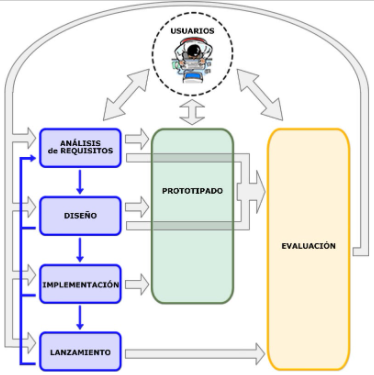
\includegraphics[width=6.0cm,height=4.0cm]{img/image_0.png}\centering

\begin{itemize}
\item Métodos de evaluación por INSPECCIÓN
\item Métodos de evaluación por INDAGACIÓN
\item Métodos de evaluación por TEST
\item Laboratorio de usabilidad
\end{itemize}
\end{frame}

\section{Inspeccion:}
%References frame
\begin{frame}
\frametitle{2.-Inspeccion:}

\begin{itemize}
\item Evaluadores analizan y explican el grado de usabilidad de un sistema basándose en la inspección o examen de la interfaz del mismo.
\item No intervienen usuarios de forma directa
\item Métodos para evaluación por inspección:\\ 1.-Heurística\\ 2.-Recorridos cognitivos\\ 3.-Recorrido de usabilidad plural\\ 4.-Revisión de Estándares
  
\end{itemize}

\begin{figure}
  \centering
  
\includegraphics[width=8.0cm,height=2.0cm]{img/image_2.jpg}
\end{figure}
\end{frame}

\section{Evaluacion Heuristica:}
%References frame
\begin{frame}
\frametitle{3.-Evaluacion Heuristica:}

\begin{itemize}
\item La comunidad IPO(Interacción persona-ordenador) presenta a la Evaluación Heurística como un método de evaluación de la usabilidad
\item A partir de unos principios previamente establecidos que se confecciona/adapta de forma individual para cada nuevo ejercicio.
\item Objetivo, medir la calidad de la interfaz de un sistema interactivo
\end{itemize}

\begin{figure}
  \centering
  
\includegraphics[width=8.0cm,height=4.0cm]{img/image_3.png}
\end{figure}
\end{frame}

\section{Metodo:}
%References frame
\begin{frame}
\frametitle{4.-Metodo:}

\begin{itemize}
 \item Preparación: el responsable\\ 1.-Determina la lista de criterios a evaluar. Puede contar con el asesoramiento de expertos.\\ 2.- Selección de los evaluadores
 \item Evaluación\\ 1.- Cada evaluador realiza individualmente una revisión de la interfaz\\ 2.- Al terminar las evaluaciones se permite a los evaluadores comunicar los resultados y sintetizarlos
  \item Síntesis Final\\ 1.- Análisis de resultados de una Evaluación Heurística
\end{itemize}

\end{frame}

\section{Los 10 principios heuristicos de Nielsen y Molich:}
%References frame
\begin{frame}
\frametitle{5.-Los 10 principios heuristicos de Nielsen y Molich:}

\begin{itemize}
\item El estado del sistemaha de estar siempre visible
\item Se ha de utilizar el lenguaje de los usuarios
\item El usuario tiene el control y libertad
\item Hay consistencia y se siguen los estandares
\item Existe prevencion de errores
\item Se minimiza la carga de la memoria del usuario
\item Existe flexibilidad y eficiencia de uso
\item Los dialogos son  esteticos y diseño minimalista
\item Al utilizar la ayuda, se reconocen, diagnostican, y se recuperan.
\item Existe ayuda y documentacion
\end{itemize}

\end{frame}

\section{Las 8 reglas de oro de Ben Schneiderman:}
%References frame
\begin{frame}
\frametitle{6.-Las 8 reglas de oro de Ben Schneiderman:}

\begin{itemize}
\item Esforzarse por la consistencia
\item Crear atajos para los usuarios frecuentes
\item Ofrecer feedback
\item Diseñar el dialogo para mostrar trabajo pendiente
\item Ofrecer una gestion sencilla de los errores
\item Permitir una facil recuperacion de acciones
\item Soportar el control por el usuario
\item Reducir la carga de memoria reciente en el usuario
\end{itemize}

\end{frame}

\section{Preparacion-Seleccion de evaluadores}
%References frame
\begin{frame}
\frametitle{7.-Preparacion-Seleccion de evaluadores}

\begin{itemize}
\item Coste-beneficio en relación a la cantidad de evaluadores necesarios para llevar a cabo una EH.
\item J. Nielsen, “How to Conduct a Heuristic Evaluation”\\
\url{http://www.useit.com/papers/heu ristic/heuristic evaluation.html}
\end{itemize}

\begin{figure}
  \centering
  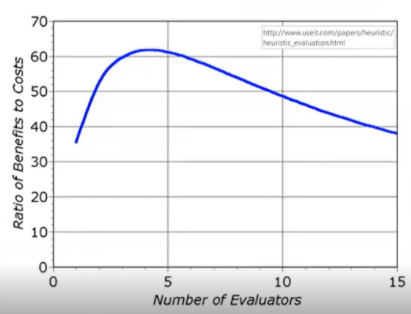
\includegraphics[width=8.0cm,height=4.0cm]{img/image_4.png}
\end{figure}
\end{frame}

\section{Revision:}
%References frame
\begin{frame}
\frametitle{8.-Revision:}

\begin{itemize}
\item IMPACTO que mide, en el subheurístico actual, la dificultad que le puede suponer al usuario superar el problema detectado en la interfaz.
\item FRECUENCIA: que indica con qué frecuencia se produce el problema.
\item PERSISTENCIA del mismo, como indicador de que una vez resuelto el problema en la parte de la interfaz en la que se ha detectado éste continuará produciéndose en otras partes de la misma.
\end{itemize}

\begin{figure}
  \centering
  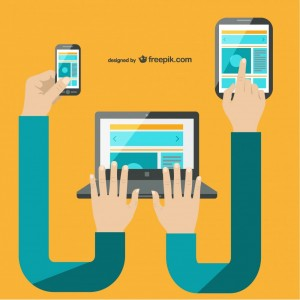
\includegraphics[width=8.0cm,height=4.0cm]{img/image_1.jpg}
\end{figure}
\end{frame}

\begin{frame}
\frametitle{8.-Revision:}

\begin{itemize}
\item Entrenamiento previo a la evaluacion\\ 1.-Conocimiento del tema e información para los evaluadores\\ 2.-Si el interfaz es del tipo de "llegar y usar" los evaluadores no necesitan esta introducción
\item Evaluacion propiamente dicha\\1.-Factores a valorar para cada principio \\2.-Forma de “puntuar” cada factor
\item Discucion\\ 1.-Puesta en común de las evaluaciones parciales \\ 2.-Este punto puede considerarse el último paso de la revisión o el primero de formar parte de la síntesis final
\end{itemize}

\end{frame}

\section{Analisis de resultados:}
%References frame
\begin{frame}
\frametitle{9.-Analisis de resultados:}

\begin{itemize}
\item CUANTITATIVO\\ 1.-Herramientas como la Estadística\\ 2.-Gráficos y funciones matemáticas de \\ 2.1.-los resultados obtenidos por un solo evaluador ("sumativa")\\ 2.2.-Los resultados obtenidos por diferentes evaluadores ("comparativa")\\ 3.-Ayudan a resumir de manera clara y precisa la ponderación de cada una de las preguntas 
\end{itemize}

\end{frame}

\begin{frame}
\frametitle{9.-Analisis de resultados:}

\begin{itemize}
\item CUALITATIVO\\ 1.-Herramientas como las Técnicas del Descubrimiento de Conocimiento en Base de Datos (Datamining)\\ 2.-Hallar de manera algorítmica (imparcial y objetiva) patrones de comportamiento desconocidos y potencialmente útiles presentes en los datos 
\end{itemize}
\begin{figure}
  \centering
  
\includegraphics[width=8.0cm,height=4.0cm]{img/image_5.jpg}
\end{figure}
\end{frame}

\section{Sintesis:}
%References frame
\begin{frame}
\frametitle{10.-Sintesis:}

\begin{itemize}
\item Documento formal de la evaluación
\item Prestar especial atención a los comentarios de los evaluadores
\item Algunos autores sugieren que es conveniente enviar un cuestionario a los evaluadores para recoger los grados de la severidad. \\ #Enumerando completamente el sistema según los problemas de usabilidad que se han descubierto, y pidiendo que clasifiquen la severidad de cada problema.
\end{itemize}

\begin{figure}
  \centering
  
\includegraphics[width=8.0cm,height=4.0cm]{img/image_7.png}
\end{figure}
\end{frame}

\section{Puntos Resaltantes:}
%References frame
\begin{frame}
\frametitle{11.-Puntos Resaltantes:}

\begin{itemize}
\item Guían a los diseñadores durante el proceso de diseño
\item Ayudan a los evaluadores a identificar problemas en las interfaces de usuario, comprobando que se respetan las reglas de usabilidad
\item Explican\\ 1.-problemas de usabilidad observados\\ 2.-porqué los usuarios cometen determinados errores

\end{itemize}

\begin{figure}
  \centering
  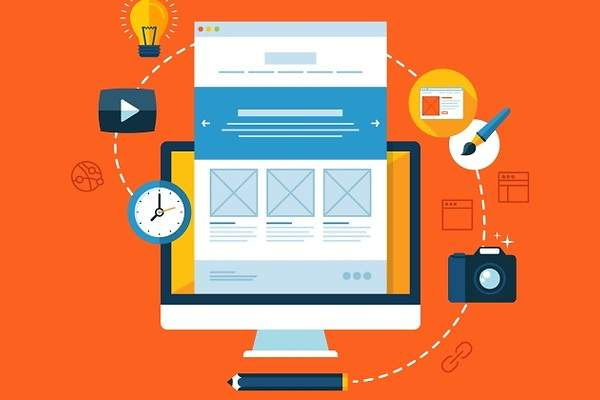
\includegraphics[width=8.0cm,height=4.0cm]{img/image_6.jpg}
\end{figure}
\end{frame}

\section{Pro y Contras:}
%References frame
\begin{frame}
\frametitle{12.-Pro y Contras:}

\begin{itemize}
\item VENTAJAS\\ 1.Económica\\ 2.Intuitiva y motivación fácil\\ 3.Poca planificación previa \\4.Utilizable en etapas tempranas  \\5.Menor tiempo que los tests de laboratorio  \\6.Realizable por evaluadores "INEXPERTOS”

\end{itemize}
\end{frame}

\begin{frame}
\frametitle{12.-Pro y Contras:}

\begin{itemize}
\item INCONVENIENTES\\ 1.Se necesitan varios evaluadores\\ 2.Difícil de realizar en interfaces complejas \\ 3.Subjetividad de los diferentes evaluadores \\ 4.Puede tender a reportar falsas alarmas \\ 5.Falta de usuarios reales\\ 6.Los evaluadores "expertos” detectan un número más alto de problemas de usabilidad
\end{itemize}
\end{frame}

\section{Propuesta de trabajo a Futuro}
%References frame
\begin{frame}
\frametitle{13.-Propuesta de trabajo a Futuro:}

\begin{itemize}
\item Dado el escenario actual de la pandemia se hace interesante poder  evaluar la usabilidad de distintas páginas web gubernamentales que cumplieron distintas funciones en este escenario y observar su nivel de usabilidad para el usuario.
Objetivo: Evaluación Heurística de portales web gubernamentales creadas en situación de pandemia tales como: \\ 1.Bono independiente\\ 2.Pase Laboral de transito.\\ 3.Bono CONFIEP.
\end{itemize}
\end{frame}

\section{Referencias:}
%References frame
\begin{frame}
\frametitle{Referencias:}
\begin{itemize}
\item Grupo Nielsen Roman: \url{https://www.nngroup.com/papers/heuristic}
\item Cuerpo de conocimiento de usabilidad: \url{http://www.usabilitybok.org/methods/p275/}
\item Interaccion persona-ordenador Evaluacion: \url{https://mpiua.invid.udl.cat/fases-mpiua/evaluacion/}
\end{itemize}
\end{frame}

\end{document}